\section*{静电场}

\subsubsection*{一. 选择题}

1. 一均匀带电球面,电荷面密度为$\sigma$,球面内电场强度处处为零,球面上面元$\d S$带有$\sigma\d S$的电荷,该电荷在球面内各点产生的电场强度\fbox{处处不为零}.

2. 下列说法中正确的是\fbox{(C)}.\pp
    (C) 场强可由$\vec{E}=\vec{F}/q$定出,其中$q$为试验电荷可负可正,$\vec{F}$为试验电荷所受的电场力.

4. 将一个试验电荷$q_0$(正电荷)放在带有负电荷的大导体附近$P$点处(如图),测得它所受的力为$F$.若考虑到电荷$q_0$不是足够小,则\fbox{(B)}.\pp
    (B) $F/q_0$比$P$点处原先的场强数值小.

图4.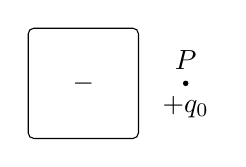
\begin{tikzpicture}
\draw[rounded corners=2pt] (0,0) rectangle (1.4,1.4);
\draw (0.7,0.7) node {$-$};
\fill (2,0.7) circle (1pt);
\draw (2,1) node {$P$};
\draw (2,0.4) node {$+q_0$};
\end{tikzpicture}
图7.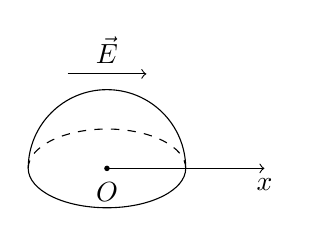
\begin{tikzpicture}
\draw (0,0) arc [start angle=0, end angle=180, x radius=1, y radius=1];
\draw[dashed] (0,0) arc [start angle=0, end angle=180, x radius=1, y radius=0.5];
\draw (0,0) arc [start angle=360, end angle=180, x radius=1, y radius=0.5];
\draw[->] (-1.5,1.2) -- (-0.5,1.2);
\draw (-1,1.5) node {$\vec E$};
\fill (-1,0) circle (1pt);
\draw (-1,-0.3) node {$O$};
\draw[->] (-1,0) -- (1,0);
\draw (1,-0.2) node {$x$};
\end{tikzpicture}
图8.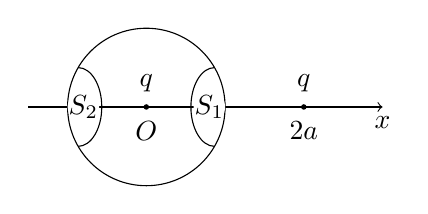
\begin{tikzpicture}
\draw (0,0) circle (1);
\fill (0,0) circle (1pt);
\draw (0,0.3) node {$q$};
\draw (0,-0.3) node {$O$};
\draw[->] (-1.5,0) -- (3,0);
\draw (3,-0.2) node {$x$};
\fill (2,0) circle (1pt);
\draw (2,0.3) node {$q$};
\draw (2,-0.3) node {$2a$};
\draw (30:1) arc [start angle=90, delta angle=180, y radius=0.5, x radius=0.3];
\fill[white] (0.8,0) circle (0.2);
\draw (0.8,0) node {$S_1$};
\draw (210:1) arc [start angle=270, delta angle=180, y radius=0.5, x radius=0.3];
\fill[white] (-0.8,0) circle (0.2);
\draw (-0.8,0) node {$S_2$};
\end{tikzpicture}

7. 一电场强度为$\vec E$的均匀电场,$\vec E$的方向沿$x$轴正方向,如图,则通过图中一半径为$R$的半球面的电场强度通量为\fbox{0}.

8. 有两个电荷都是$+q$的点电荷,相距为$2a$.今以左边的点电荷所在处为球心,以$a$为半径作一球形高斯面.在球面上取两块相等的小面积$S_1$和$S_2$,其位置如图所示.设通过$S_1$和$S_2$的电场强度通量分别为$\varPhi_1$和$\varPhi_2$,通过整个球面的电场强度通量为$\varPhi_S$,则\fbox{$\varPhi_1<\varPhi_2, \varPhi_S=q/\varepsilon_0$}.

\subsubsection*{二. 填空题}

\subsubsection*{三. 计算题}
